\newpage
\section{Understanding Mobility Based on GPS Data~\cite{Zheng:2008:UMB:1409635.1409677}} \label{lect1}

\subsection{Summary} \label{lect1-sum}

\subsubsection{Context}

A considerable amount of research studies have focussed on detecting significant locations
in the user trajectory data, predicting future locations of a user or recognising user specific 
activity at a particular location. On the contrary, classifying user GPS trajectories 
based on transportation modes has not received substantial attention. Knowledge regarding 
the transportation modes is significant in order to provide pervasive computing systems with
meaningful context information. 

\subsubsection{Problem}

To date, the transportation mode classification, relies on manual labelling by the users or  
utilised GSM radio signals, which could only discriminate between simple motions such as moving
and being stationary. On the other hand, identification methods based on trivial approaches such
as velocity based classification leads to inherent errors due to the frequency at which users 
switch the travel modes. The velocity of the travel modes is also influenced by traffic conditions 
and weather. In this paper the user GPS trajectories are used to understand and 
distinguish between users transportation mode, such as walking, driving or taking a bus based on 
supervised learning.  

\begin{figure}[h]
\centering
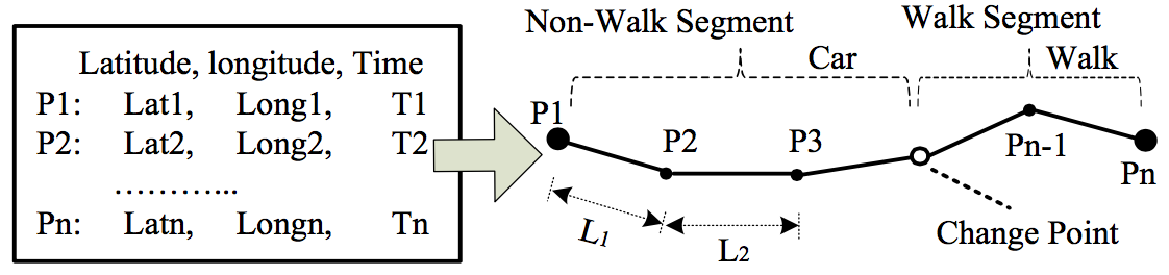
\includegraphics[width=0.5\textwidth]{tm1.pdf}
\caption{GPS logs and transportation mode prediction~(From~\cite{Zheng:2008:UMB:1409635.1409677})}
\end{figure}

\subsubsection{Contributions}

\paragraph{Results\newline}

In order to infer the transportation mode, the authors identify a set of novel features beyond 
simple velocity and acceleration. These features along with a post processing algorithm are 
robust to the traffic condition and contain significant information of users motion. The technique 
was evaluated using GPS logs collected by 65 users over a time period of 10 months. The authors 
evaluated the proposed approach by considering various combinations of the suggested features
and achieved a prediction accuracy of 72.8~\%.   

\paragraph{Approach\newline}

The framework to infer the transportation mode consists of an offline learning stage and a online
processing stage. In the offline learning part, the GPS trajectories are partitioned into segments
depending on the direction change points. The individual segments are than utilised to extract 
several features which are used to train a classification model for the online inference stage.\newline

When the GPS trajectory comes, it is first partitioned into segments from which several features such as 
direction change rate, velocity change rate, stop rate and heading direction are extracted. 
Using these features, the inference model is utilised to predict the transportation mode for
a given segment in a probabilistic manner. As a classification model, decision tree is used based on 
a change point based segmentation method. The change points are grouped into several clusters using
a density-based clustering algorithm. The derived clusters are used to construct an undirected graph
with nodes as individual cluster and edges being the transportation between nodes. A spatial index is
built over the graph to improve the efficiency of accessing information of each node and edge. Finally,
the probability distribution is calculated of different transportation modes on each edge.    

change point based segmentation method, variable traffic conditions, graph based post processing 
algorithm, independent of any additional database of road networks or POI's. Independent of sensor data
such as GSM signal, heart rate, and map information like road networks and bus stops. Therefore
can be deployed in a range of web applications. Non user-specific model. 


\subsection{Discussion} \label{lect1-disc}

The contribution of the above paper is a methodology to infer the mobility mode, given raw GPS
data logs. The non-user specific model presented in the paper is independent of external sensors 
such as GSM signals, heart rate and map information like road networks and bus stops. The change 
point based segmentation method devised by the authors is proved to be robust to variable traffic
conditions. Thus, it can be deployed in a range of web applications.      


\begin{itemize}

\item The technique presented, involves an offline training phase which uses the extracted features 
to generate the online transportation mode inference model. It would have been interesting to quantify 
the data required and computational time/complexity involved at the offline stage to arrive at a sufficient
online prediction accuracy.

\item The paper states that the devised approach is a non-user specific model. However, sufficient 
evaluation of the experimental results regarding generalisation of user specific models is not presented
in the paper. 

\item The authors derive several features from the raw GPS logs to train the inference model. Although, 
it is evident that a combination of certain features results in a sufficient prediction accuracy, a 
combination of a particular features reduces the accuracy. The reasoning behind such a behaviour is lacking 
in the evaluation section. 

\item Considering majority of the population owning a smart phone have Internet connection, it will be
interesting to map the extracted segments to road maps and points of interests in the training phase 
to increase the prediction accuracy. 

\item The segmentation technique described, extracts segments from consecutive GPS points. However, there
will exist some segments which do not offer any valuable information for feature extraction. It will 
also be interesting to extract the only segments providing valuable information based on other attributes.   
\end{itemize}